% This contents of this file will be inserted into the _Solutions version of the
% output tex document.  Here's an example:

% If assignment with subquestion (1.a) requires a written response, you will
% find the following flag within this document: <SCPD_SUBMISSION_TAG>_1a
% In this example, you would insert the LaTeX for your solution to (1.a) between
% the <SCPD_SUBMISSION_TAG>_1a flags.  If you also constrain your answer between the
% START_CODE_HERE and END_CODE_HERE flags, your LaTeX will be styled as a
% solution within the final document.

% Please do not use the '<SCPD_SUBMISSION_TAG>' character anywhere within your code.  As expected,
% that will confuse the regular expressions we use to identify your solution.

\def\assignmentnum{3 }
\def\assignmenttitle{XCS234 Assignment \assignmentnum}
\input{macros}
\begin{document}
\pagestyle{myheadings} \markboth{}{\assignmenttitle}

% <SCPD_SUBMISSION_TAG>_entire_submission

This handout includes space for every question that requires a written response.
Please feel free to use it to handwrite your solutions (legibly, please).  If
you choose to typeset your solutions, the |README.md| for this assignment includes
instructions to regenerate this handout with your typeset \LaTeX{} solutions.
\ruleskip

\LARGE
1.b
\normalsize

% <SCPD_SUBMISSION_TAG>_1b
\begin{answer}
  % ### START CODE HERE ###

  \textbf{Last eval trajectory for IQL with $\zeta=0.2$, PointmassEasy-v0}

  \begin{center}
    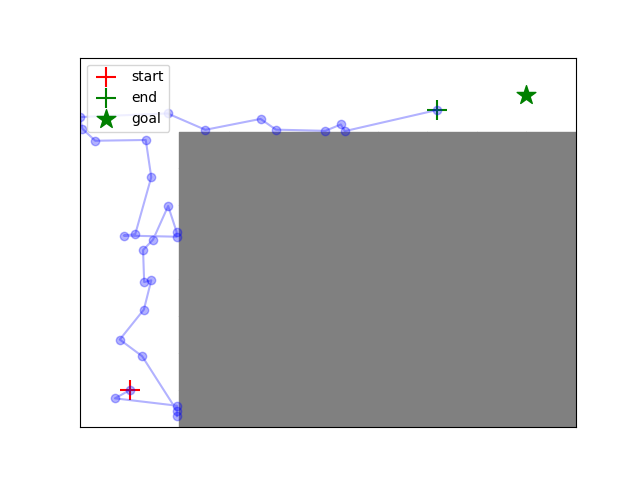
\includegraphics[width=0.7\textwidth]{../src/submission/data/hw3_iql_zeta_0.2_rnd_PointmassEasy-v0_21-03-2026_22-32-31/eval_last_traj.png}

    \begin{tabular}{lc}
      \hline
      Average Return & $-22.395$\\
      Std Return & $7.355$\\
      \hline
    \end{tabular}
  \end{center}

  \textbf{Last eval trajectory for IQL with $\zeta=0.9$, PointmassEasy-v0}

  \begin{center}
    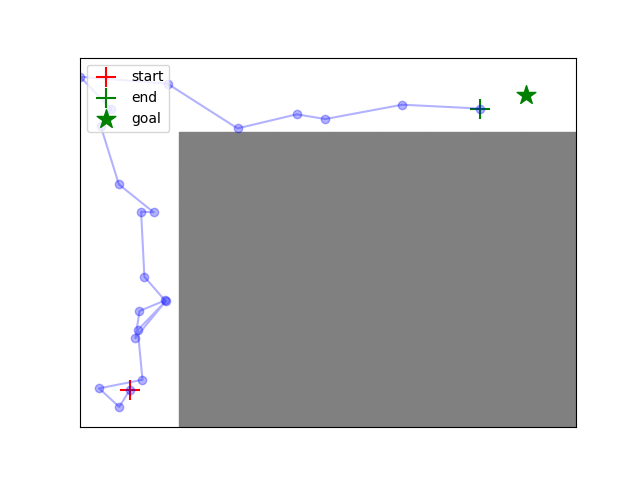
\includegraphics[width=0.7\textwidth]{../src/submission/data/hw3_iql_zeta_0.9_rnd_PointmassEasy-v0_21-03-2026_23-56-14/eval_last_traj.png}


    \begin{tabular}{lc}
      \hline
      Average Return & $-19.14$\\
      Std Return & $5.43$\\
      \hline
    \end{tabular}
  \end{center}

  % ### END CODE HERE ###
\end{answer}
% <SCPD_SUBMISSION_TAG>_1b
\clearpage

\LARGE
1.c
\normalsize

% <SCPD_SUBMISSION_TAG>_1c
\begin{answer}
  % ### START CODE HERE ###

  \textbf{Last eval trajectory for IQL with RND exploration, $\zeta=0.9$, PointmassMedium-v0}

  \begin{center}
    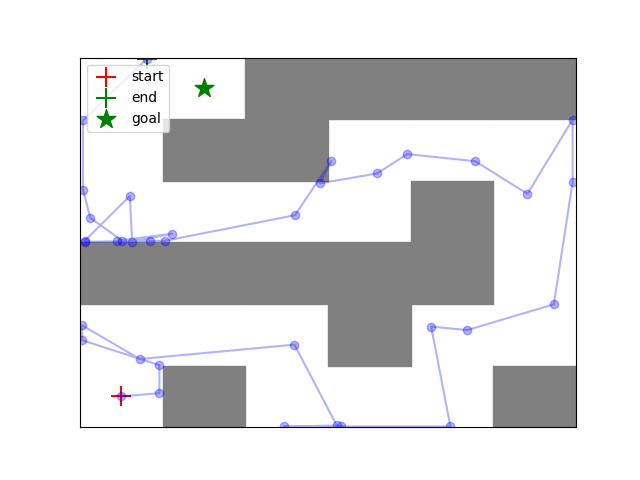
\includegraphics[width=0.7\textwidth]{../src/submission/data/hw3_iql_zeta_0.9_rnd_PointmassMedium-v0_22-03-2026_00-23-56/eval_last_traj.png}

    \begin{tabular}{lc}
      \hline
      Average Return & $-46.364$\\
      Std Return & $14.615$\\
      \hline
    \end{tabular}
  \end{center}

  \textbf{Last eval trajectory for IQL with random exploration, $\zeta=0.9$, PointmassMedium-v0}

  \begin{center}
    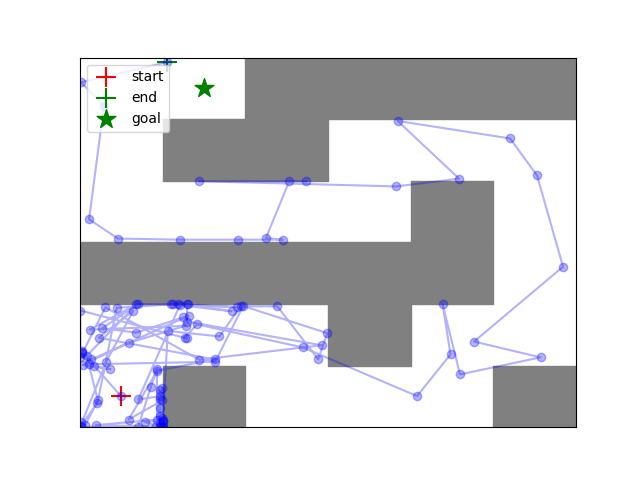
\includegraphics[width=0.7\textwidth]{../src/submission/data/hw3_iql_zeta_0.9_random_PointmassMedium-v0_22-03-2026_02-03-47/eval_last_traj.png}

    \begin{tabular}{lc}
      \hline
      Average Return & $-78.0$\\
      Std Return & $21.711$\\
      \hline
    \end{tabular}
  \end{center}

  % ### END CODE HERE ###
\end{answer}
% <SCPD_SUBMISSION_TAG>_1c
\clearpage


\LARGE
2.b
\normalsize

% <SCPD_SUBMISSION_TAG>_2b
\begin{answer}
  % ### START CODE HERE ###

  \textbf{Last eval trajectories for CQL $\alpha=0.0$, PointmassHard-v0, runs 1 and 2}

  \begin{center}
    \includegraphics[width=0.45\textwidth]{../src/submission/data/hw3_cql_alpha_0.0_rnd_PointmassHard-v0_22-03-2026_02-18-24/eval_last_traj.png}
    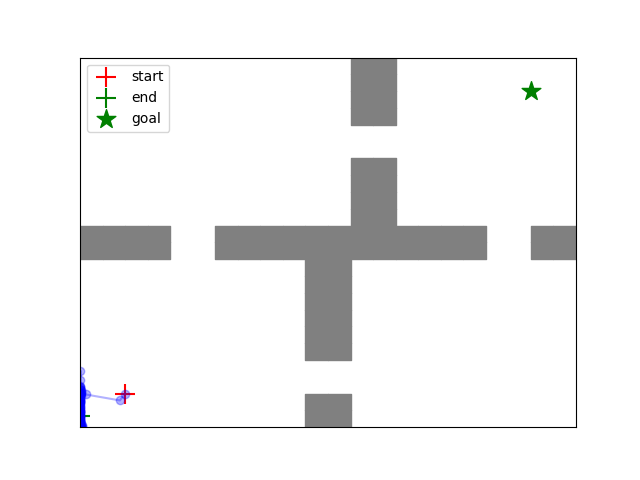
\includegraphics[width=0.45\textwidth]{../src/submission/data/hw3_cql_alpha_0.0_rnd_PointmassHard-v0_22-03-2026_09-20-42/eval_last_traj.png}

    \begin{tabular}{llcc}
      \hline
      Run & & Average Return & Std Return \\
      \hline
      Run 1 & & $-78.0$ & $21.711$ \\
      Run 2 & & $-100.0$ & $0.0$ \\
      \hline
    \end{tabular}
  \end{center}

  % TODO: Run a 3rd seed for alpha=0.0 and add its eval_last_traj.png + row here.

  \textbf{Last eval trajectories for CQL $\alpha=0.1$, PointmassHard-v0, runs 1 and 2}

  \begin{center}
    \includegraphics[width=0.45\textwidth]{../src/submission/data/hw3_cql_alpha_0.1_rnd_PointmassHard-v0_22-03-2026_02-18-43/eval_last_traj.png}
    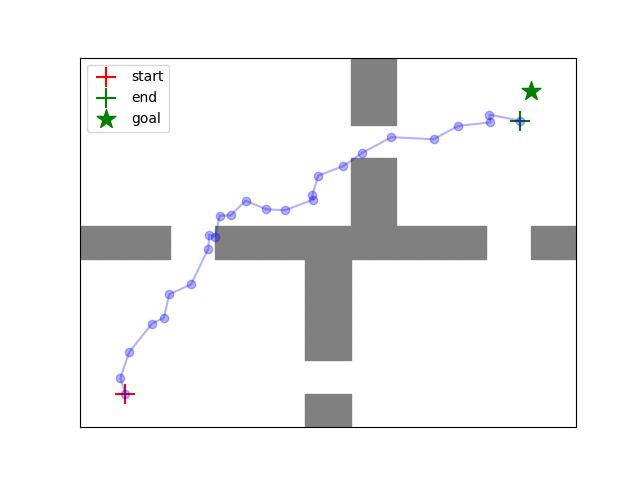
\includegraphics[width=0.45\textwidth]{../src/submission/data/hw3_cql_alpha_0.1_rnd_PointmassHard-v0_22-03-2026_09-30-47/eval_last_traj.png}

    \begin{tabular}{llcc}
      \hline
      Run & & Average Return & Std Return \\
      \hline
      Run 1 & & $-39.60$ & $7.014$ \\
      Run 2 & & $-100.0$ & $0.0$ \\
      \hline
    \end{tabular}
  \end{center}

  % TODO: Run a 3rd seed for alpha=0.1 (RND) and add its eval_last_traj.png + row here.

  % ### END CODE HERE ###
\end{answer}
% <SCPD_SUBMISSION_TAG>_2b
\clearpage

\LARGE
2.c
\normalsize

% <SCPD_SUBMISSION_TAG>_2c
\begin{answer}
  % ### START CODE HERE ###

  \textbf{Last eval trajectories for CQL $\alpha=0.1$, RND exploration, PointmassHard-v0, runs 1 and 2}

  \begin{center}
    \includegraphics[width=0.45\textwidth]{../src/submission/data/hw3_cql_alpha_0.1_rnd_PointmassHard-v0_22-03-2026_02-18-43/eval_last_traj.png}
    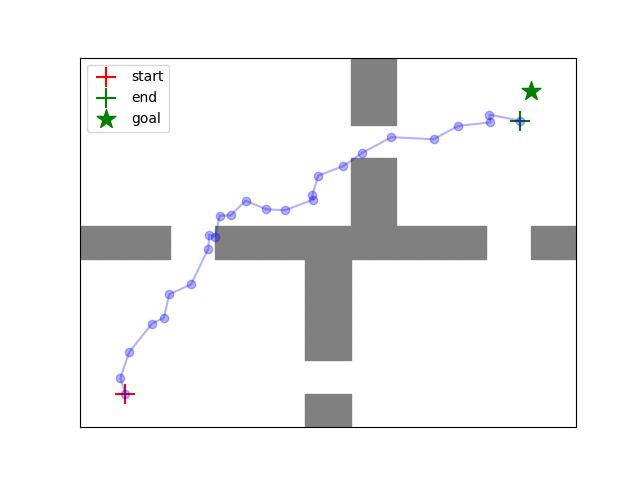
\includegraphics[width=0.45\textwidth]{../src/submission/data/hw3_cql_alpha_0.1_rnd_PointmassHard-v0_22-03-2026_09-30-47/eval_last_traj.png}

    \begin{tabular}{llcc}
      \hline
      Run & & Average Return & Std Return \\
      \hline
      Run 1 & & $-39.60$ & $7.014$ \\
      Run 2 & & $-100.0$ & $0.0$ \\
      \hline
    \end{tabular}
  \end{center}

  % TODO: Add 3rd run image for alpha=0.1 RND here.

  \textbf{Last eval trajectories for CQL $\alpha=0.1$, random exploration, PointmassHard-v0, runs 1 and 2}

  \begin{center}
    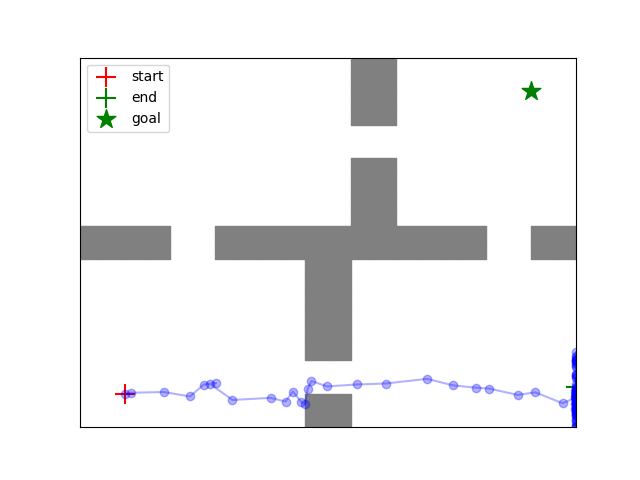
\includegraphics[width=0.45\textwidth]{../src/submission/data/hw3_cql_alpha_0.1_random_PointmassHard-v0_22-03-2026_02-19-02/eval_last_traj.png}
    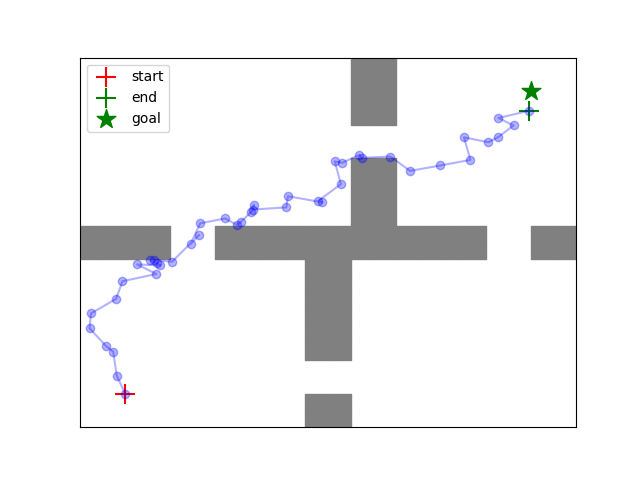
\includegraphics[width=0.45\textwidth]{../src/submission/data/hw3_cql_alpha_0.1_random_PointmassHard-v0_22-03-2026_09-41-34/eval_last_traj.png}

    \begin{tabular}{llcc}
      \hline
      Run & & Average Return & Std Return \\
      \hline
      Run 1 & & $-36.148$ & $4.494$ \\
      Run 2 & & $-100.0$ & $0.0$ \\
      \hline
    \end{tabular}
  \end{center}

  % TODO: Add 3rd run image for alpha=0.1 random here.

  % ### END CODE HERE ###
\end{answer}
% <SCPD_SUBMISSION_TAG>_2c
\clearpage

% <SCPD_SUBMISSION_TAG>_entire_submission

\end{document}
